\documentclass{beamer}
\beamertemplatenavigationsymbolsempty
\usecolortheme{beaver}
\setbeamertemplate{blocks}[rounded=true, shadow=true]
\setbeamertemplate{footline}[page number]

\usepackage{amsmath,amssymb,amsfonts}
\usepackage{graphicx}
\usepackage{tikz}

\title{Sequential Neural Score Estimation: Likelihood-Free Inference with Conditional Score Based Diffusion Models}
\author{Louis Sharrock, Jack Simons, Song Liu, Mark Beaumont}
\institute{Talk by Gleb Karpeev}
\date{}

\begin{document}

\begin{frame}
\titlepage
\end{frame}

\begin{frame}{Simulation-Based Inference Problem}

\begin{block}{Problem Setup}
Given a prior $p(\theta)$ and a simulator $p(x|\theta)$, infer posterior:
\begin{equation*}
p(\theta|x_{obs}) = \frac{p(x_{obs}|\theta)p(\theta)}{p(x_{obs})}
\end{equation*}
\end{block}

\begin{block}{Key Challenge}
\begin{itemize}
    \item Likelihood $p(x|\theta)$ is intractable
    \item Can sample from simulator but cannot evaluate density
    \item Standard MCMC and VI methods are not applicable
\end{itemize}
\end{block}

\begin{block}{Applications}
Neuroscience, evolutionary biology, epidemiology, climate science, cosmology, econometrics
\end{block}

\end{frame}

\begin{frame}{Existing SBI Approaches}

\begin{block}{Neural Density Estimation Methods}
\begin{itemize}
    \item SNPE: Learn posterior $q_\psi(\theta|x) \approx p(\theta|x)$ using normalizing flows
    \item SNLE: Learn likelihood $q_\psi(x|\theta) \approx p(x|\theta)$, then use MCMC
    \item SNRE: Learn likelihood ratio $r(x,\theta) = p(\theta|x)/p(\theta)$
\end{itemize}
\end{block}

\begin{block}{Limitations}
\begin{itemize}
    \item Normalizing flows require invertibility constraints
    \item GANs suffer from training instability
    \item Need for careful architectural design
\end{itemize}
\end{block}

\end{frame}

\begin{frame}{Score-Based Diffusion Models: Key Idea}

\begin{block}{Score Function}
Instead of modeling density $p(\theta|x)$, model its gradient:
\begin{equation*}
s(\theta) = \nabla_\theta \log p(\theta|x)
\end{equation*}
\end{block}

\begin{block}{Advantages}
\begin{itemize}
    \item No normalization constant needed
    \item Architectural flexibility (no invertibility required)
    \item Stable training (no adversarial objectives)
    \item Proven success in generative modeling
\end{itemize}
\end{block}

\end{frame}

\begin{frame}{Neural Posterior Score Estimation (NPSE)}

\begin{block}{Forward Noising Process}
Gradually add noise to transform $p(\theta|x)$ to tractable $\pi(\theta) = \mathcal{N}(0,I)$:
\begin{equation*}
d\theta_t = f(\theta_t, t)dt + g(t)dw_t
\end{equation*}
\end{block}

\begin{block}{Backward Process}
Time-reversal generates samples from posterior:
\begin{equation*}
d\bar{\theta}_t = \left[-f(\bar{\theta}_t, T-t) + g^2(T-t)\nabla_\theta \log p_{T-t}(\bar{\theta}_t|x)\right]dt + g(T-t)dw_t
\end{equation*}
\end{block}

\begin{block}{Key Insight}
Only need score $\nabla_\theta \log p_t(\theta_t|x)$, not the density itself!
\end{block}

\end{frame}

\begin{frame}{NPSE: Training and Sampling}

\begin{block}{Score Matching Objective}
Train neural network $s_\psi(\theta_t, x, t) \approx \nabla_\theta \log p_t(\theta_t|x)$ by minimizing:
\begin{equation*}
\mathcal{J}_{post}^{DSM}(\psi) = 
\frac{1}{2}\int_0^T \lambda_t \mathbb{E}_{p_{t|0}(\theta_t|\theta_0)p(x|\theta_0)p(\theta_0)} \left[\|s_\psi(\theta_t, x, t) - \nabla_{\theta_t}\log p_{t|0}(\theta_t|\theta_0)\|^2\right]dt
\end{equation*}
\end{block}

\begin{block}{Sampling via Probability Flow ODE}
\begin{equation*}
\frac{d\theta_t}{dt} = \left[f(\theta_t, t) - \frac{1}{2}g^2(t)s_\psi(\theta_t, x_{obs}, t)\right]
\end{equation*}
Starting from $\theta_T \sim \mathcal{N}(0,I)$, integrate backward to obtain $\theta_0 \sim p(\theta|x_{obs})$
\end{block}

\end{frame}

\begin{frame}{Visualization: Two Moons Example}

\begin{figure}
    \centering
    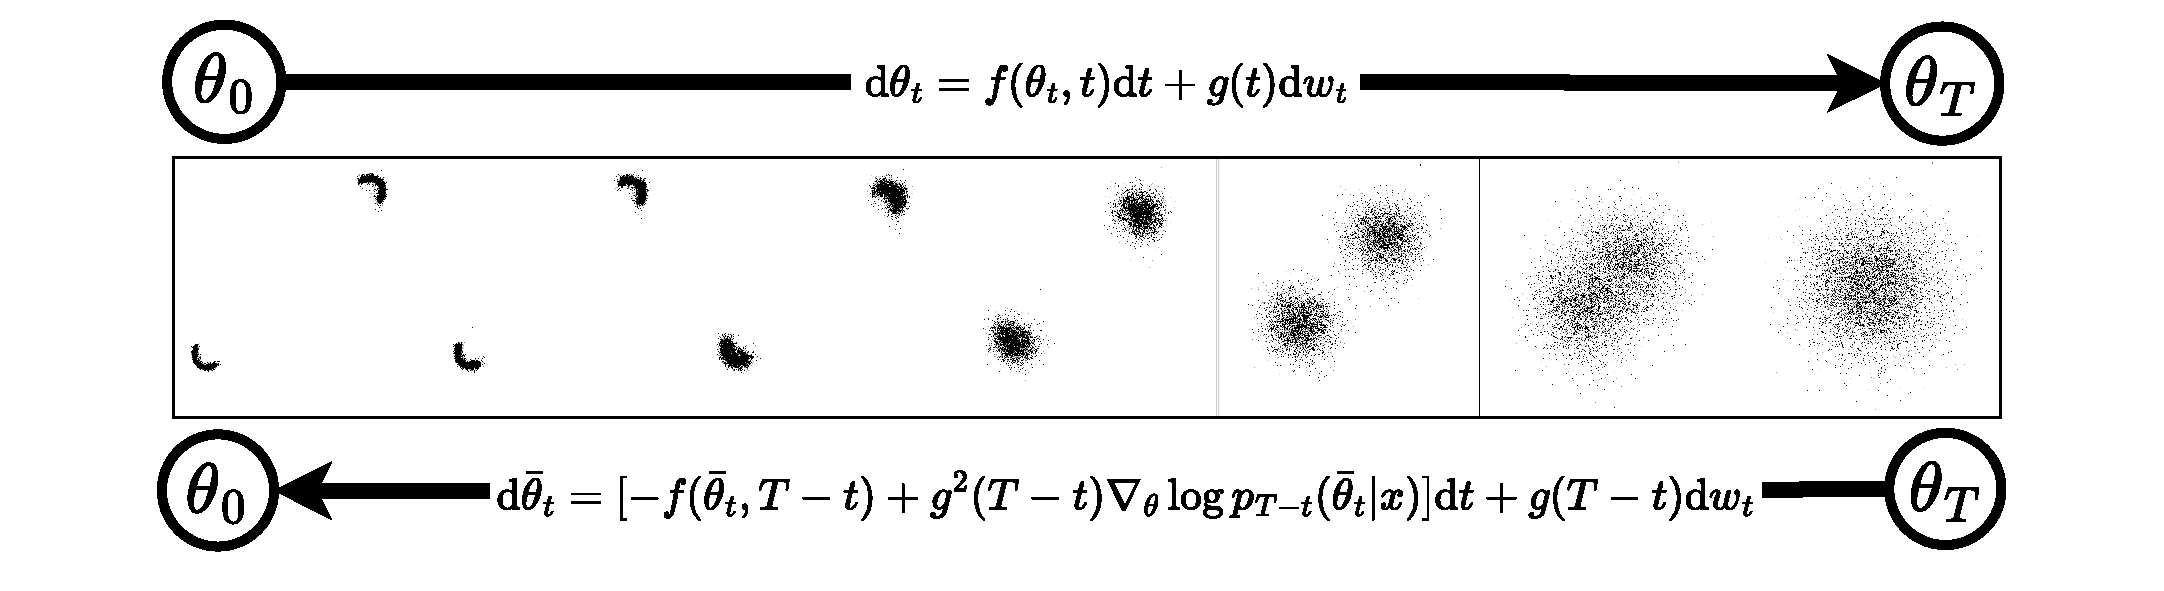
\includegraphics[width=0.95\linewidth]{fig1.pdf}
    \caption{Forward process transforms posterior to Gaussian; backward process (with learned scores) generates posterior samples}
    \label{fig:twomoons}
\end{figure}

\end{frame}

\begin{frame}{Sequential Training: Motivation}

\begin{block}{Problem with Non-Sequential Approach}
\begin{itemize}
    \item Sample $\theta_i \sim p(\theta)$ uniformly from prior
    \item Most samples far from posterior at $x_{obs}$
    \item Inefficient use of limited simulation budget
\end{itemize}
\end{block}

\begin{block}{Sequential Solution}
\begin{itemize}
    \item Adaptively guide simulations using current posterior approximation
    \item Focus computational resources on informative regions
    \item Use proposal distribution $\tilde{p}^r(\theta)$ that concentrates near $x_{obs}$
\end{itemize}
\end{block}

\begin{block}{Central Challenge}
How to correct for mismatch between proposal posterior and true posterior?
\end{block}

\end{frame}

\begin{frame}{Truncated Sequential NPSE (TSNPSE)}

\begin{block}{Key Idea: Truncated Priors}
In round $r$, define truncated prior using highest probability region:
\begin{equation*}
\bar{p}^r(\theta) \propto p(\theta) \cdot \mathbb{I}\{\theta \in \text{HPR}_\epsilon(p_\psi^{r-1}(\theta|x_{obs}))\}
\end{equation*}
\end{block}

\begin{block}{Proposal as Mixture}
\begin{equation*}
\tilde{p}^r(\theta) = \frac{1}{r}\sum_{s=0}^{r-1} \bar{p}^s(\theta)
\end{equation*}
where $\bar{p}^0(\theta) = p(\theta)$
\end{block}

\begin{block}{Elegant Result}
If we don't truncate regions with posterior support, then $\tilde{p}^r(\theta) \propto p(\theta)$ within support.\\
No importance weight correction needed!
\end{block}

\end{frame}

\begin{frame}{Alternative Sequential Approaches}

\begin{block}{SNPSE-A: Post-hoc Correction}
\begin{itemize}
    \item Generate samples from proposal posterior
    \item Resample using importance weights $w_i \propto p(\theta_i)/\tilde{p}^r(\theta_i)$
    \item Issue: Approximation error when learned proposal differs from true
\end{itemize}
\end{block}

\begin{block}{SNPSE-B: Weighted Loss Function}
\begin{itemize}
    \item Include importance weights in loss: $\frac{p(\theta_0)}{\tilde{p}^r(\theta_0)} \|\cdot\|^2$
    \item Theoretically correct but high variance
    \item Unstable training
\end{itemize}
\end{block}

\begin{block}{SNPSE-C: Score-space Correction}
\begin{itemize}
    \item Correct via score decomposition
    \item Requires multiple additional approximations
\end{itemize}
\end{block}

\end{frame}

\begin{frame}{Benchmark Results: Non-Sequential Methods}

\begin{figure}
    \centering
    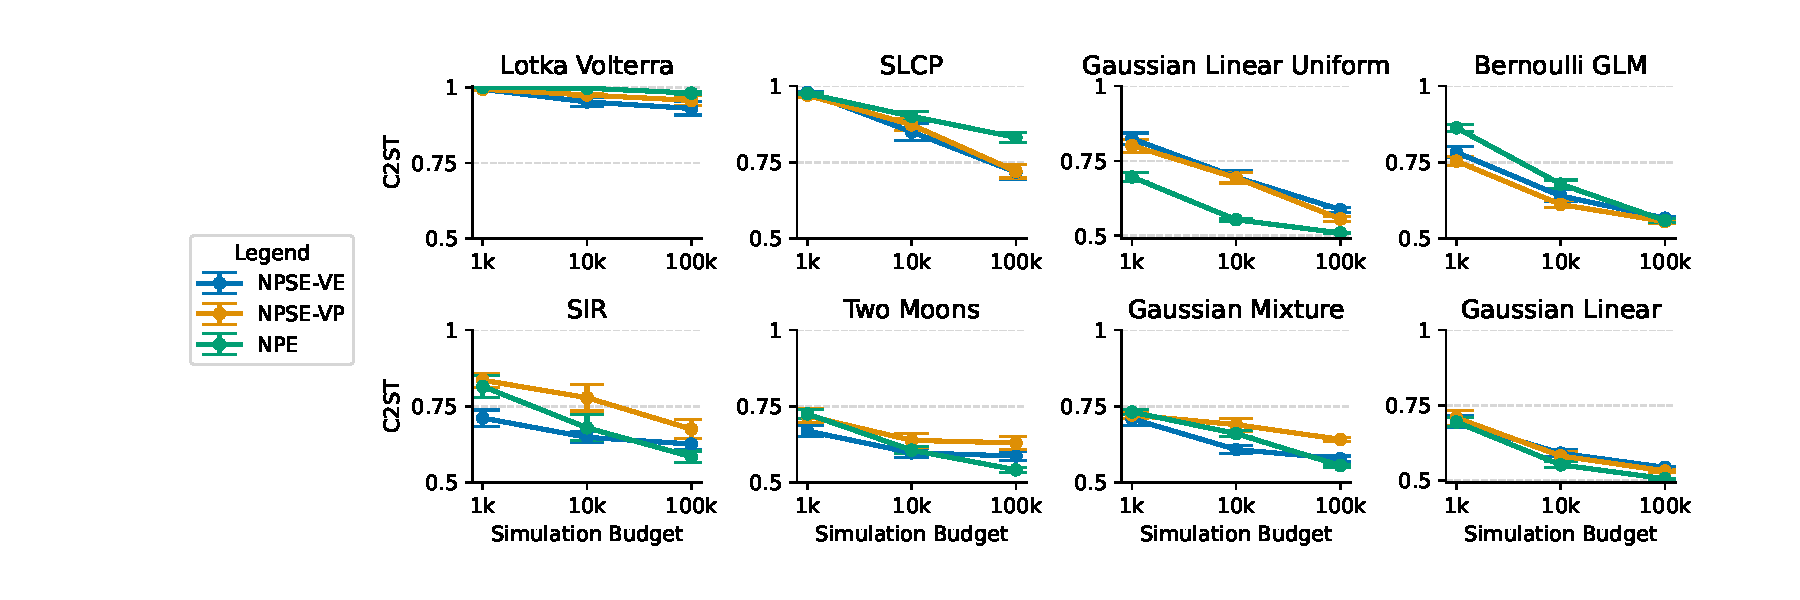
\includegraphics[width=0.95\linewidth]{all_subplots_nonseq.pdf}
    \caption{C2ST scores on 8 benchmarks (lower is better, 0.5 is perfect). NPSE competitive with NPE across tasks.}
    \label{fig:nonseq}
\end{figure}

\end{frame}

\begin{frame}{Benchmark Results: Sequential Methods}

\begin{figure}
    \centering
    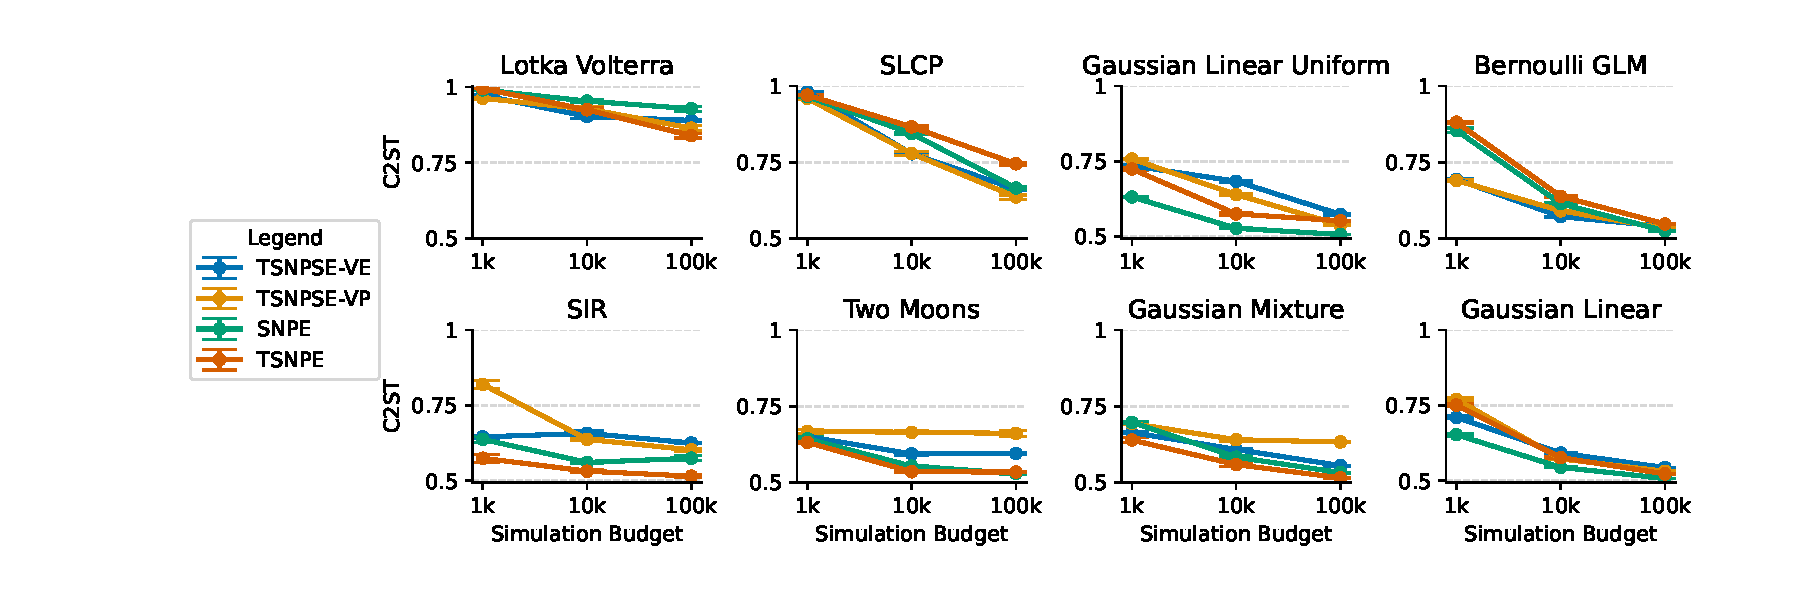
\includegraphics[width=0.95\linewidth]{all_subplots_seq.pdf}
    \caption{TSNPSE outperforms SNPE and TSNPE on challenging high-dimensional tasks (SLCP, Lotka-Volterra)}
    \label{fig:seq}
\end{figure}

\end{frame}

\begin{frame}{Real-World Application: Pyloric Network}

\begin{block}{Problem Characteristics}
\begin{itemize}
    \item 31 parameters governing neural dynamics
    \item 18 summary statistics from voltage traces
    \item $>$99\% of prior samples produce invalid statistics
    \item Extremely challenging for SBI methods
\end{itemize}
\end{block}

\begin{block}{TSNPSE Performance}
\begin{itemize}
    \item 9 rounds, 190k total simulations
    \item 81\% valid statistics in final round (vs $<$60\% for TSNPE)
    \item Posterior predictive matches observed data
    \item Marginals comparable to SNVI and TSNPE
\end{itemize}
\end{block}

\end{frame}

\begin{frame}{Pyloric Results: Visualizations}

\begin{figure}
    \centering
    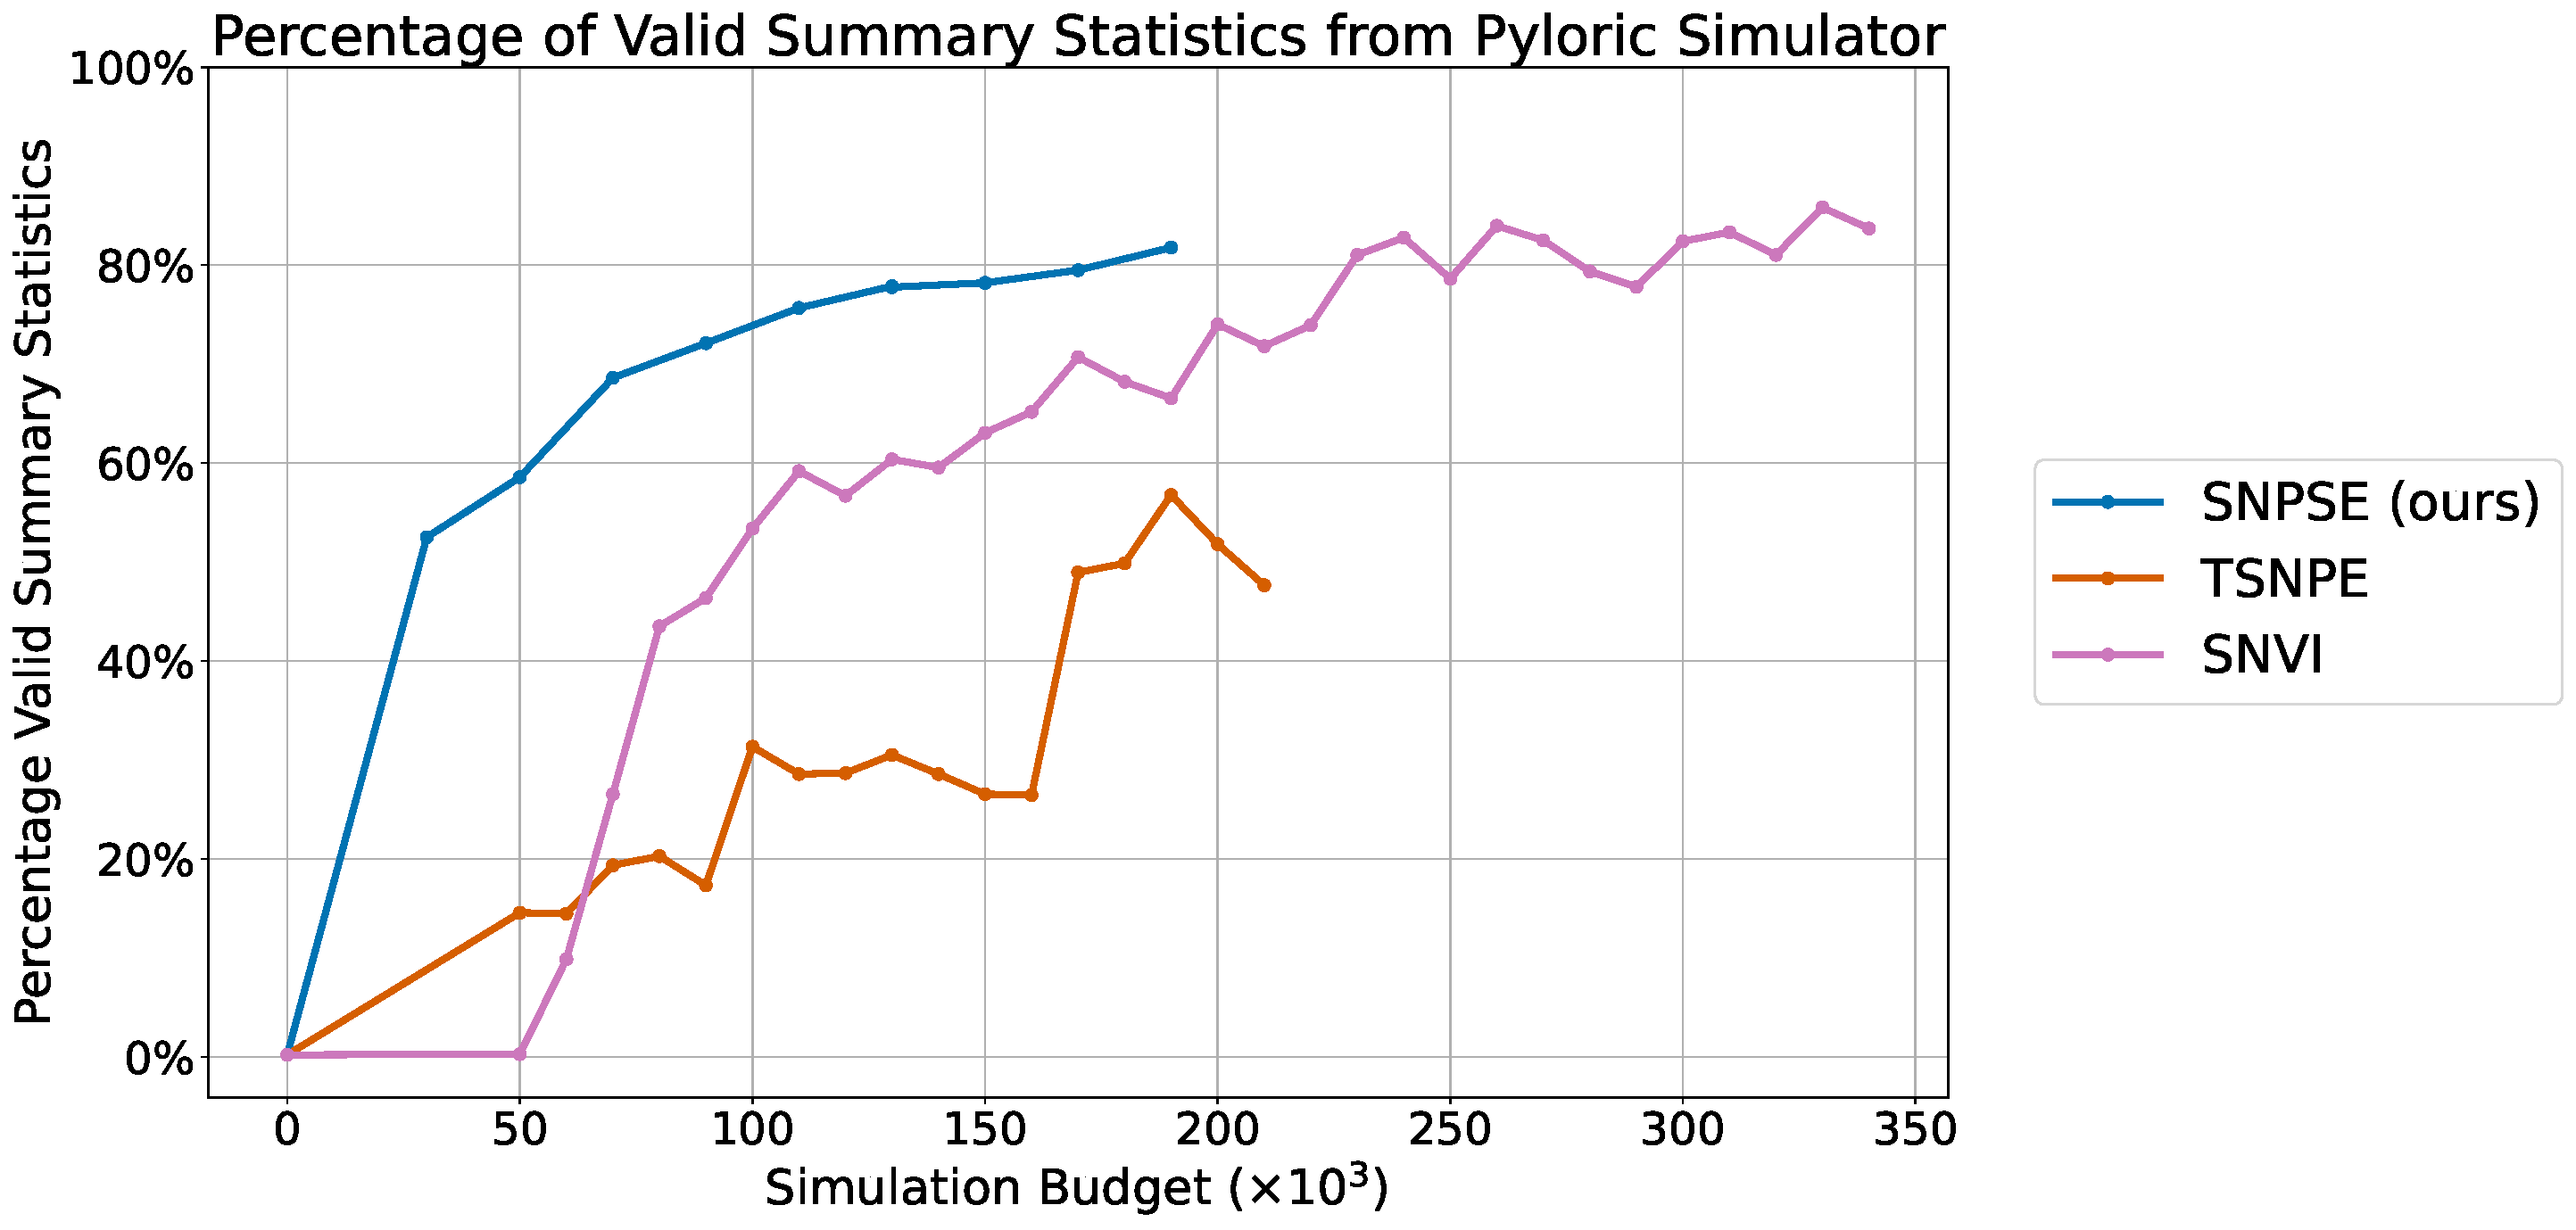
\includegraphics[width=0.9\linewidth]{pyloric_acceptance_2.pdf}
    \caption{Top: Posterior mean predictive vs observation. Bottom: Percentage of valid statistics improves significantly with sequential focusing.}
    \label{fig:pyloric}
\end{figure}

\end{frame}

\begin{frame}{Conclusion}

\begin{block}{Key Contributions}
\begin{itemize}
    \item First application of score-based diffusion models to SBI
    \item TSNPSE: principled sequential training via truncated priors
    \item No importance weight corrections needed
    \item Architectural flexibility without normalizing flow constraints
\end{itemize}
\end{block}

\begin{block}{Empirical Results}
\begin{itemize}
    \item Comparable or superior to SNPE on benchmarks
    \item Particularly strong on high-dimensional problems
    \item Successful on challenging real-world neuroscience application
\end{itemize}
\end{block}

\begin{block}{Future Directions}
Sequential variants of flow matching, specialized architectures for SBI, theoretical guarantees
\end{block}

\end{frame}

\end{document}